\chapter{Concepts and State of the Art}\label{ch:2}

\epigraph{The problem with object-oriented languages is they've got all this
implicit environment that they carry around with them. You wanted a banana but what you got was a gorilla holding the banana and the entire jungle.}{Joe Armstrong}

In this section we will discuss the most important concepts that are going to
be used in this paper.


\section{Fundamental Concepts}

\subsection{Modeling, Metamodeling}


	Object-oriented programming is a paradigm which appeared in the
early '60 \cite{wiki:oop} and is based on the concept of defining object and
relationships between them. With the rapid growth of software system
object-oriented design has become a non-trivial problem even for small systems,
thus the need of tools that can assist us in analyzing our design. The use of
object technologies in detecting problems is called object-oriented analysis.

	Modeling, as defined in the dictionary \cite{dictionary:modeling}, is the
representation, often mathematical, of a process, concept, or operation of a system, 
often implemented by a computer program.  There is no general accepted
definition for this term, but for the purpose of this paper we can see a model
as a simplified version of a reality. As there can be many types of maps for the
same territory depending on the purpose (riding a bike, traveling to cities,
sightseeing) there can also be many types of models for the same system depending from which angle
we want view the system. Figure \ref{fig:CatModel} illustrates the idea.

\begin{figure}
\centering
\scalebox{0.3}{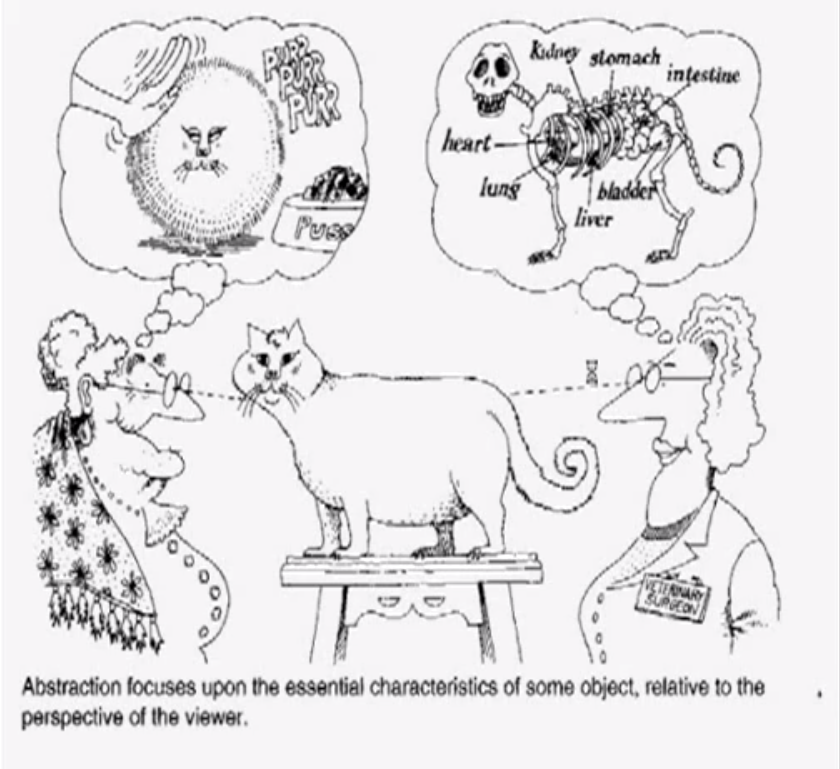
\includegraphics{img/concepts/CatModel.png}}
\caption{The same cat but from different perspectives\label{fig:CatModel}}
\end{figure}	
	
	In order to be able to work with models software analysis tools need to be able
to understand and represent them, thus the need of a way to describe models. For
this the concept of metamodeling has been introduced. The prefix meta- indicates 
an abstraction of a concept \cite{wiki:meta}. Formally, metamodel is an abstract 
syntax which governs the representation of a class of models. One of the most
common metamodels used in object oriented design (modeling) is UML
\cite{book:UMLDistilled}. One is able to describe it's object oriented system by
simply showing and describing the most important entities, i.e objects, and how
they interact with each other. In  figure \ref{fig:umlMetamodel} we have
representation of the XML metamodel described using UML.

   \begin{figure}
		\centering
		\scalebox{0.3}{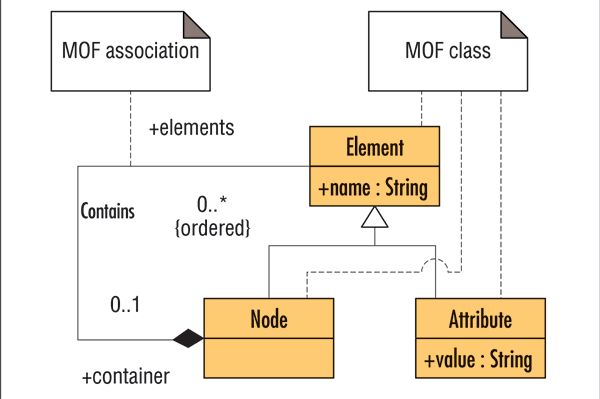
\includegraphics{img/concepts/umlMetamodel.png}}
		\caption{XML metamodel\label{fig:umlMetamodel}}
	\end{figure}

	A very common case with tools is that people want them aggregated in one larger
tool. In order to do this we will need to define a way to describe software
analysis tools. As software analysis tools use metamodels for describing models,
it natural to assume that we will need a meta-metamodel in order to describe a
metamodel. Thus a metamodel is also governed by a strict set of rules that form
a meta-metamodel. One can easily see that the definition is recursive and we
could continue with it indefinitely. In time many meta-metamodels have been
implemented in order to solve different problems (e.g Ecore, GME, KM3, \ldots{}
etc). For the purpose of this application we have used a simple meta-metamodel
based on three elements: 
	\begin{itemize}
		\item Entity --- represents a generalization of a package, type, method, 
field 
		\item Property ---
		\item Groups ---
	\end{itemize}
%%% must add explications for properties and groups and entities
	
	The figure \ref{fig:metamodel} represents a summary of the basic concepts
presented so far.
	 

\begin{figure}
\centering
\scalebox{0.5}{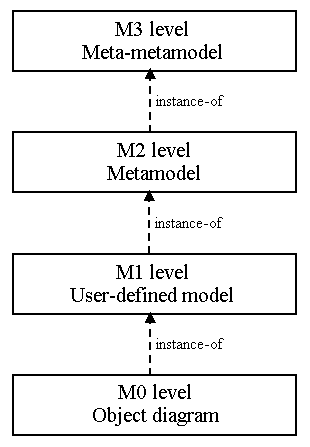
\includegraphics{img/concepts/metamodel.png}}
\caption{Models and Metamodels\label{fig:metamodel}}
\end{figure}
		
		
\subsection{Java Metaprogramming}

	
	As mentioned above a model is nothing more or less than a simplified version of
a reality/system. In case of software analysis tools this system is actually a
program. In order to be able to manipulate programs (models) we need specific
language support for this type of programming, also called metaprogramming
\cite{website:metaprogramming}. 

	Many languages have different ways and levels of supporting metaprogramming,
in C++ this is done by using the template system (template metaprogramming), in
Java this is done by using the reflection API provided by the compiler and/or by using the annotation
language feature which allows metadata processing, i.e the ability to add
information to your code so that it can be used later for generating boiler
plate code or by enforcing constraints that can be verified at compile-time or
run-time. \cite{book:ThinkingInJava} 
	
	The most common annotations that are used in java are:
	\begin{enumerate}
	  \item \textbf{@Override} -- indicates that the current method is an
 (re)implementation of method from the base class.
  
	  \item \textbf{@Deprecated} -- usually used in frameworks and indicates that
	  the entity will be removed in feature updates and support for it is no longer
 provided.
 
	  \item \textbf{@SuppressWarnings} -- stop the compiler from adding annoying
 warning.
	\end{enumerate}
	
	The syntax for defining an annotation is quite straight forward:
	\small
	\begin{lstlisting}[language=Java,numbers=left]
		public @interface myAnnotationName {}
	\end{lstlisting}
	\normalsize{}
	Of course, as we love recursion, we have meta-annotations which describe
	
	The more complex part comes wen we want to associate some semantics to our
annotations. This is usually done by defining an \textbf{annotation processor},
i.e a compiler plugin which will be invoked when our annotation(s) have been
discovered by the compiler. After each annotation processor has finished some
extra code might have been generated or some annotations might have been
expanded in other annotations or both, in this case the compiler starts
processing the code and invoking the annotation processors again as can be
seen in figure \ref{fig:annProc}.
	 In order to be able to define an annotation processor
	
	
	
		
	
\begin{figure}
\centering
\scalebox{0.8}{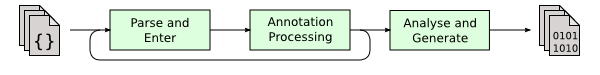
\includegraphics{img/concepts/javac-flow.png}}
\caption{The compiler process with annotation processing\label{fig:annProc}}
\end{figure}
		

\section{CodePro}



